\chapter{Introducción}
\thispagestyle{empty}

\section{Definición del problema}
La identificación facial ha adquirido gran relevancia durante la última década. La revolución del aprendizaje profundo y los sistemas automáticos de reconocimiento facial han llevado a una expansión del mercado desde los campos de la aplicación de la ley y la ciencia forense hasta áreas en el sector privado:comercio minorista, aplicaciones multimedia o seguridad. Además, el desarrollo de la tecnología de imagen ha mejorado tanto la calidad como la disponibilidad de datos fotográficos,lo que también ha contribuido a la aplicación de técnicas de identificación multimodal mediante el uso de modelos faciales en 3D o imágenes médicas \cite{1,2}.

Las técnicas de identificación normalmente son realizadas por expertos con o sin la ayuda de sistemas automáticos. Los expertos analizan los datos y evalúan las características anatómicas de un individuo desconocido para compararlas con las de uno o varios individuos conocidos. Actualmente existen cuatro métodos de comparación facial reconocidos: análisis morfológico, superposición, foto-antropometría y comparación holística \cite{3}.
Para que este análisis sea confiable y concluyente, los datos (fotografías faciales), deben estar en unas condiciones adecuadas (calidad, resolución, enfoque o iluminación) y la escena (punto de vista de la cámara, pose de la cabeza, expresión facial) debe ser lo más neutral y representativa posible. Estos requisitos nos aseguran que los rasgos faciales sean más fieles a las características anatómicas del individuo, y por tanto, permiten que las técnicas de identificación sean más robustas.

Muchos estudios han identificado limitaciones en los actuales métodos de reconocimiento automático. Los principales factores más desafiantes son la pose, la iluminación, la expresión y la variación en la edad \cite{4,6}. Sin embargo también existen otros factores importantes como la oclusión, el género o la etnia \cite{5,7}.

Uno de los factores más determinantes es la distorsión de perspectiva \cite{8} // que es una deformación o transformación de un objeto y su entorno que difiere significativamente de cómo se vería el objeto con una longitud focal normal, debido a la escala relativa de las características cercanas y distantes //. En nuestro caso, el objeto es el rostro de un individuo, por ejemplo, podríamos observar la deformación de los rasgos faciales (orejas, nariz o forma de la cara) debido a la cercanía de la cámara al sujeto durante la adquisición de la fotografía \cite{12} (ver Figura \ref{fig1}). La distorsión de perspectiva tiene un efecto negativo en los sistemas de reconocimiento automático \cite{9,10,11}, lo que a su vez puede dificultar la identificación precisa de individuos. La distorsión de perspectiva está estrechamente relacionada con la distancia cámara-sujeto (subject-to-camera distance, SCD en adelante), de hecho, la relación es de decremento logarítmico, esto significa que, valores pequeños de SCD corresponden con una mayor distorsión, mientras que la distorsión disminuye conforme el SCD aumenta \cite{23}. Por esta razón, este TFG trata sobre la estimación del SCD en fotografías faciales.

\begin{figure}[h]
	\centering
	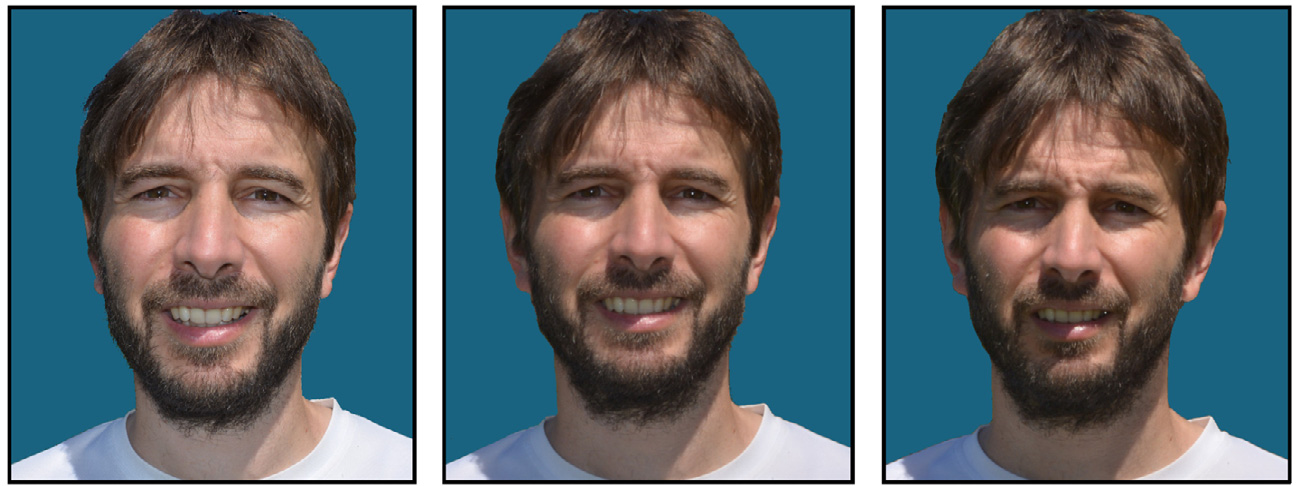
\includegraphics[scale=0.25]{imagenes/cap1/facial_distortion.png}
	\caption{Efectos de la distorsión de perspectiva en características faciales de fotografías realizadas a diferentes SCD: 0.5 m, 1 m y 3 m. Estos efectos varían en relación a la distancia y son independientes de la longitud focal \cite{14}}
	\label{fig1}
\end{figure}


La estimación del SCD en imágenes faciales abre la posibilidad a cuantificar las diferencias en la distorsión entre dos conjuntos de imágenes, y además, la posibilidad de reproducir las condiciones originales de la escena cuando hay disponibles modelos faciales 3D o restos esqueléticos. Esta última característica se considera esencial tanto para técnicas de identificación manual como automáticas, ya que mejoran la credibilidad de las comparaciones faciales mediante la medición y control de una mayor fuente de incertidumbre.

El único método totalmente automatizado para estimar el SCD en fotografías faciales, hasta la fecha, se llama FacialSCDnet \cite{14}. Este método utiliza una arquitectura basada en deep learning (VGG-16) para procesar fotografías faciales y estimar el SCD. La arquitectura VGG-16 es ampliamente reconocida por sus habilidades para aprender tareas. Las capas convolucionales del modelo VGG-16, usadas en FacialSCDnet, son pre-entrenadas con el conjunto de datos ImageNet y se reajustan (fine-tuning) con un conjunto de datos diseñado específicamente para la tarea de estimar el SCD. Este conjunto de datos específico se compone de una parte sintética y una parte real.

El propósito de este TFG es mejorar el método actual del estado del arte en la estimación automática del SCD. Para ello, se plantea mejorar el proceso de generación de una base de datos sintética de manera que haya modelos 3D más completos (de cuerpo entero y poses distintas) con fondos e iluminación más realistas.
Por otro lado, se explorarán mejoras adicionales como un cambio de framework que optimice los procesos de entrenamiento, el uso de un sistema de image augmentation que emplee GPU, o el desarrollo y uso de nuevas arquitecturas que mejoren los resultados.


\section{Motivación}
En el ámbito forense, el principal foco recae sobre la determinación de la identidad humana cuando existe información esquelética \cite{22}. En las últimas décadas, los antropólogos han centrado su atención en mejorar las técnicas para realizar una identificación más precisa. En este contexto, la estimación del SCD juega un papel crucial, ya que, si estimamos el SCD con fiabilidad, podemos recrear la imagen con los restos esqueléticos (aplicando el valor del SCD). A continuación, realizamos las comparaciones anatómicas mediante la superposición craneofacial \cite{21} para identificar si se corresponde con la misma persona (ver Figura \ref{fig2}). Si los parámetros de adquisición entre ambas imágenes (normal y esquelética) son distintos entonces dificultaría el análisis morfológico \cite{23}.

\begin{figure}[h]
	\centering
	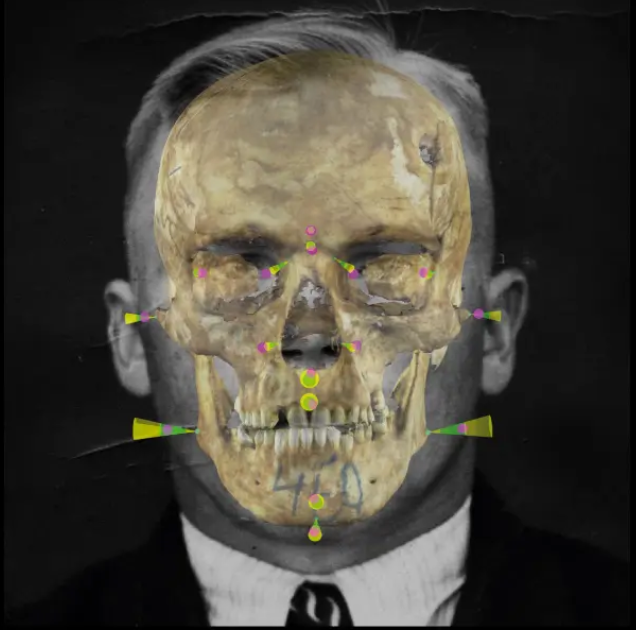
\includegraphics[scale=0.25]{imagenes/cap1/skull_superimposition.png}
	\caption{Ejemplo de superposición craneofacial \cite{23}.}
	\label{fig2}
\end{figure}


Por otra parte, sabemos que el SCD y la distorsión de perspectiva (PD) tienen una relación de decremento logarítmico \cite{23}. Esto significa que, para cuantificar el nivel de distorsión entre dos imágenes, bastaría con estimar el SCD para cada una de ellas, y mediante la siguiente fórmula hayamos el porcentaje de distorsión:

$$PD(\%) = (\frac{B'}{A'} - 1) \times 100$$

donde A' y B' son las proyecciones, en el sensor de la cámara, de los objetos A y B.

- Mitigar los efectos de la distorsión  DISCO


\section{Objetivos}
El objetivo general de este Trabajo de Fin de Grado (TFG) consiste en desarrollar un método adecuado para abordar el problema de la estimación de la distancia cámara-sujeto (SCD) en  fotografías faciales. Para el desarrollo del proyecto, dividiremos el objetivo general en una serie de objetivos parciales:
\begin{enumerate}
    \item Realizar un análisis exhaustivo del estado del arte para la estimación del SCD en fotografías faciales.
    \item Generar un conjunto de datos sintético de mayor calidad (modelos 3D más completos de cuerpo entero y poses distintas, con fondos e iluminación más realistas)
    \item Realizar un estudio experimental que permita validar los enfoques propuestos y extraer conclusiones sobre su aplicabilidad al problema.
    \item Desarrollar y entrenar con nuevas arquitecturas que mejoren los resultados
    \item Usar tecnologías más recientes que mejoren los tiempos de aprendizaje y los resultados obtenidos
\end{enumerate}